\documentclass[a4paper,10pt]{article}
\usepackage[utf8]{inputenc}
\usepackage{amsmath}
\usepackage{amssymb}
\usepackage{graphicx}
%für quellcode
\usepackage{listings} 

\newcommand{\image}[3]{\begin{figure}[h]
                            \includegraphics[#1]{#3}
                            \caption{#2}
                       \end{figure}
                       }

\lstset{
    language = octave
}
%begin{lstlisting}

\begin{document}
%########################################
%		Titel
%########################################
\begin{center}
    \section*{Mustererkennung 8.Übungszettel}
     \today
\end{center}
$ $
\newline
\begin{tabular}{r|l l}
    Name & Alexander Hinze-Hüttl & Kevin Pandura\\
    Matrikelnummer & 4578322 & 4562742\\
\end{tabular}
\newline
$ $
\newline
\newline
%########################################
%		Ende
%########################################

\section*{Aufgabe 1}
\subsection*{a}
	\texttt{
0.3,0.5,0.4 -> f15 (Tautologie) \\
-0.8, -0.6, 0.5 -> f1 (AND)\\
0.7,0.6,-1 -> f8 (NOR)}\\
\\
\textbf{Code:}\\
	\begin{lstlisting}
0;
function e = exec1(w1,w2,w3,t1,t2)
  if ((w1*t1 + w2*t2 + w3) >= 0)
     e = 1;
   else
     e = 0;
   endif
endfunction

function f = getBoolFunc(w1,w2,w3)
  e1 = exec1(w1,w2,w3,0,0);
  e2 = exec1(w1,w2,w3,0,1);
  e3 = exec1(w1,w2,w3,1,0);
  e4 = exec1(w1,w2,w3,1,1);
  
  f = e1*2^0 + e2*2^1 + e3*2^2 + e4*2^3;
endfunction

f1 = getBoolFunc(0.3,0.5,0.4);
f2 = getBoolFunc(-0.8,-0.6,0.5);
f3 = getBoolFunc(0.7,0.6,-1);

fprintf("[0.3,0.5,0.4] -> f%d\n", f1);
fprintf("[-0.8, -0.6, 0.5] -> f%d\n", f2);
fprintf("[0.7,0.6,-1] -> f%d\n", f3);
	\end{lstlisting}
\subsection*{b}
	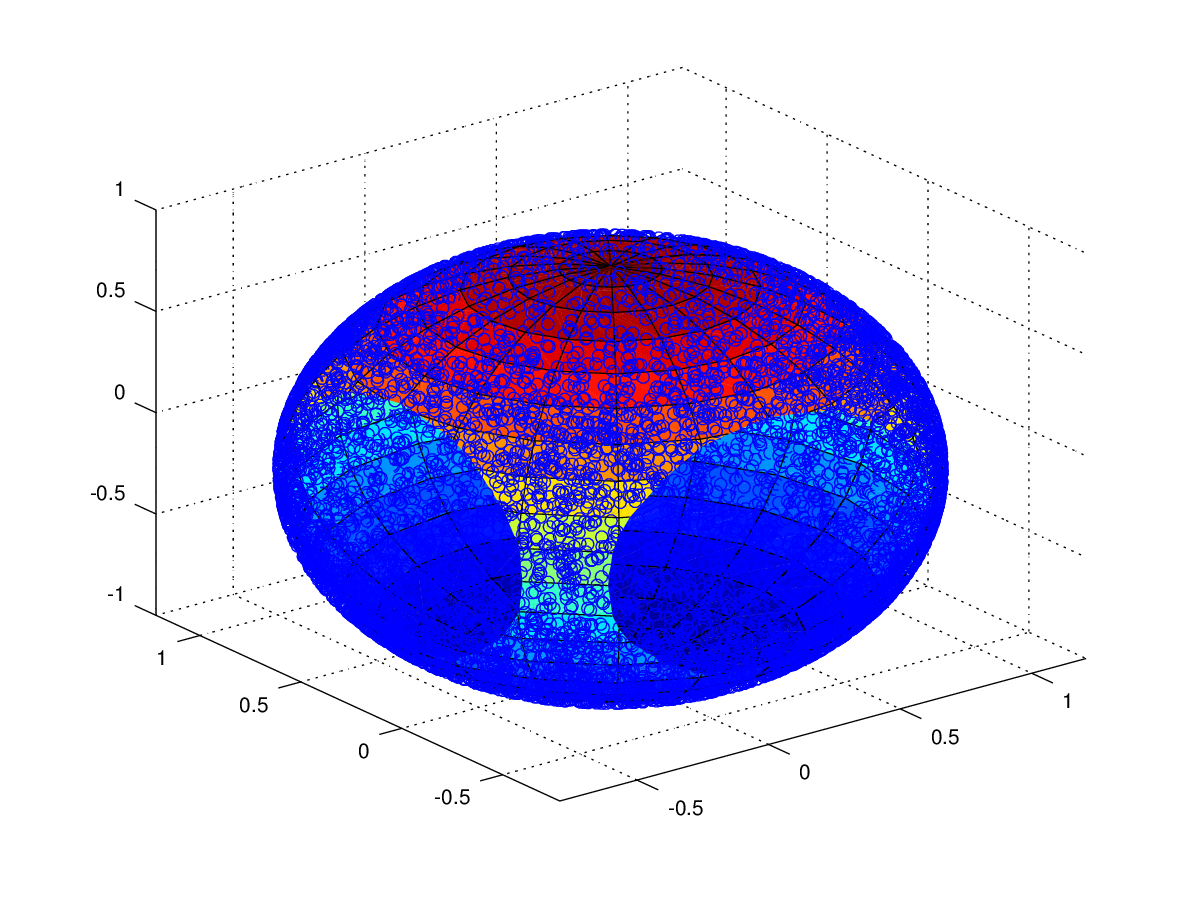
\includegraphics[scale=0.5]{sphere_1.png}\\
	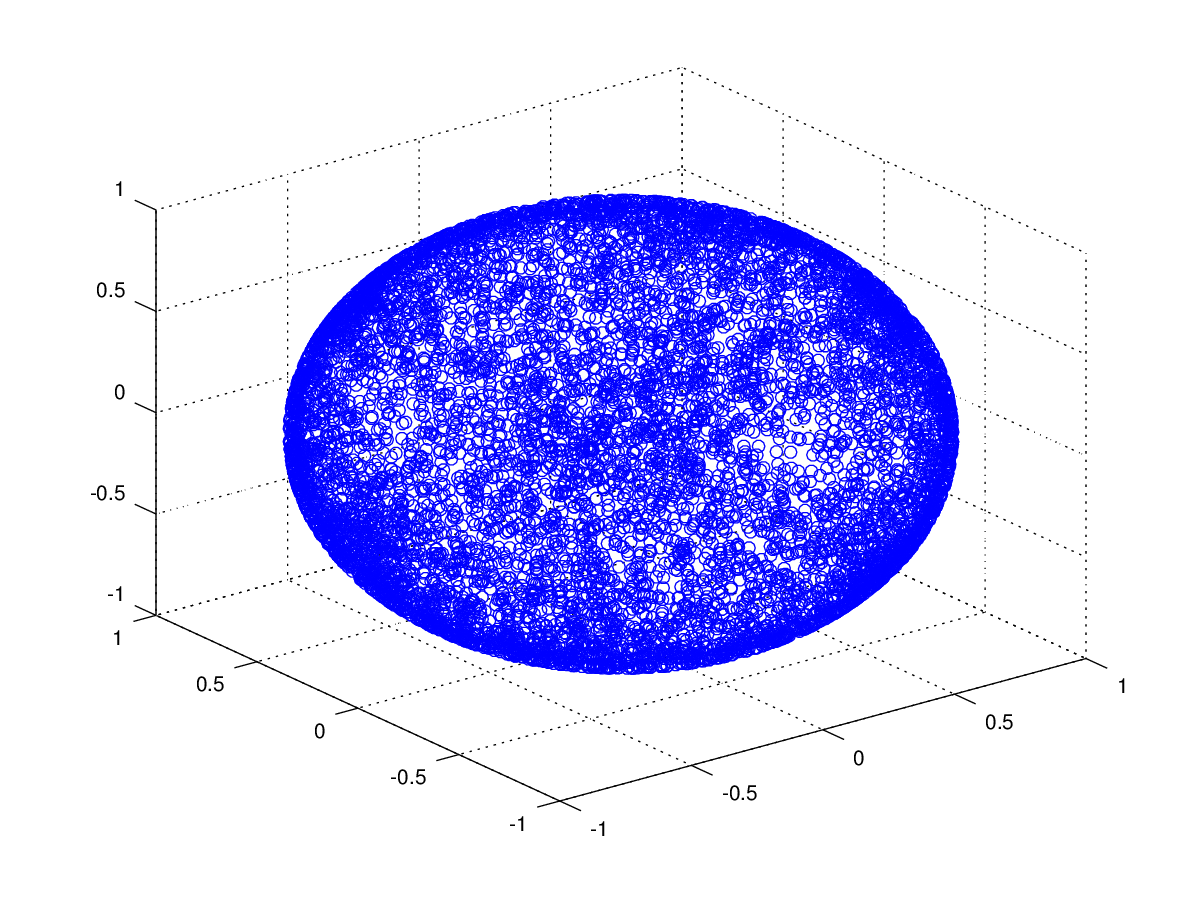
\includegraphics[scale=0.5]{sphere.png}
	\textbf{Code:}\\
	\begin{lstlisting}
0;
points = zeros(10000,3);
[h,w] = size(points);

for i = 1:h
  points(i,:) = -1 + (2)*rand(1,3);
  points(i,:) = points(i,:)/norm(points(i,:));
  scatter3(points(i,1),points(i,2),points(i,3)); hold on;
endfor
sphere;
	\end{lstlisting}
\subsection*{c}
	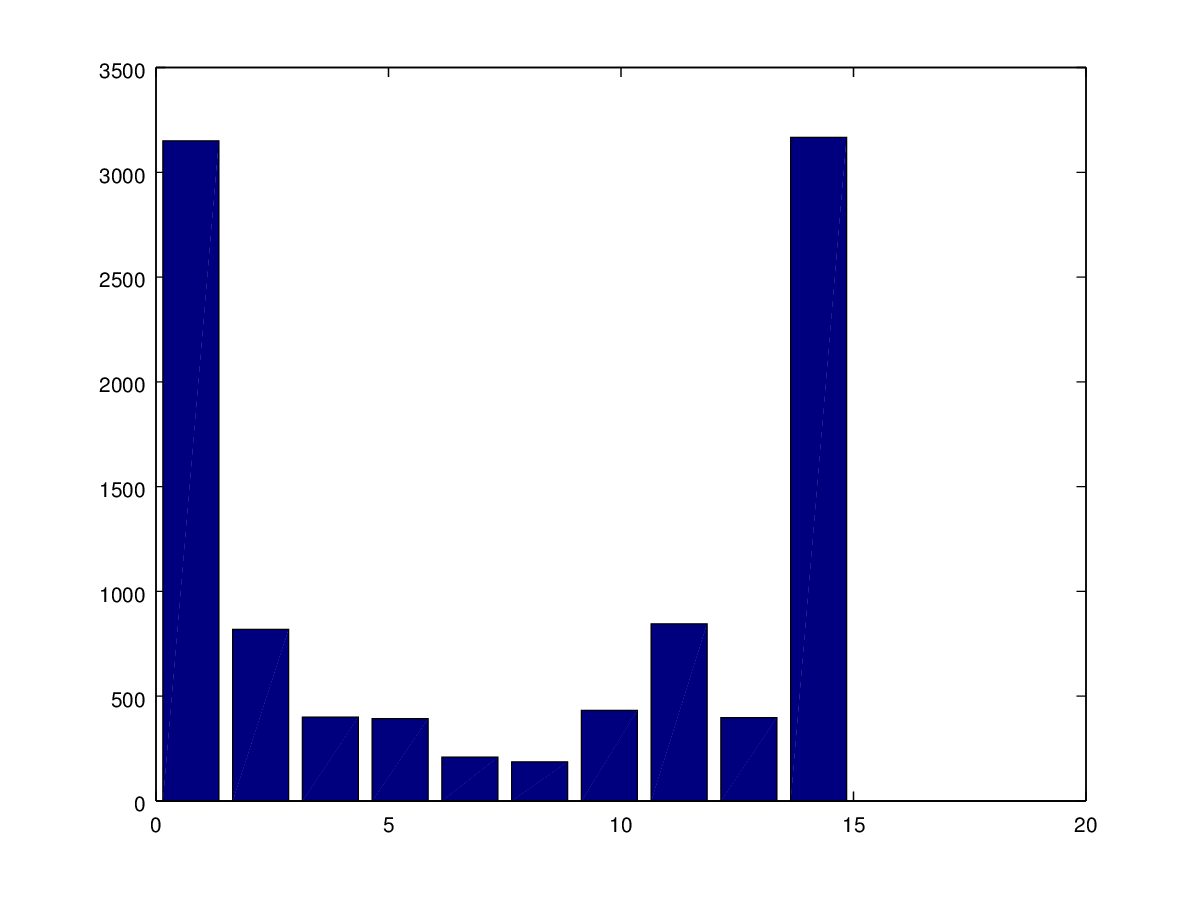
\includegraphics[scale=0.5]{boolfunctions.png}\\
	\textbf{Code:}\\
	\begin{lstlisting}

n = 10000;
rndweights = zeros(n,3);
functions = zeros(n,1);
[h,w] = size(rndweights);

for i = 1:h
  rndweights(i,:) = -1 + 2*rand(1,3);
endfor

for i = 1:h
  w1 = rndweights(i,1);
  w2 = rndweights(i,2);
  w3 = rndweights(i,3);
  f = getBoolFunc(w1,w2,w3); ... Funktione aus 1a
  functions(i,1) = f;
endfor
hist(functions,16);
	\end{lstlisting}
\subsection*{d}
	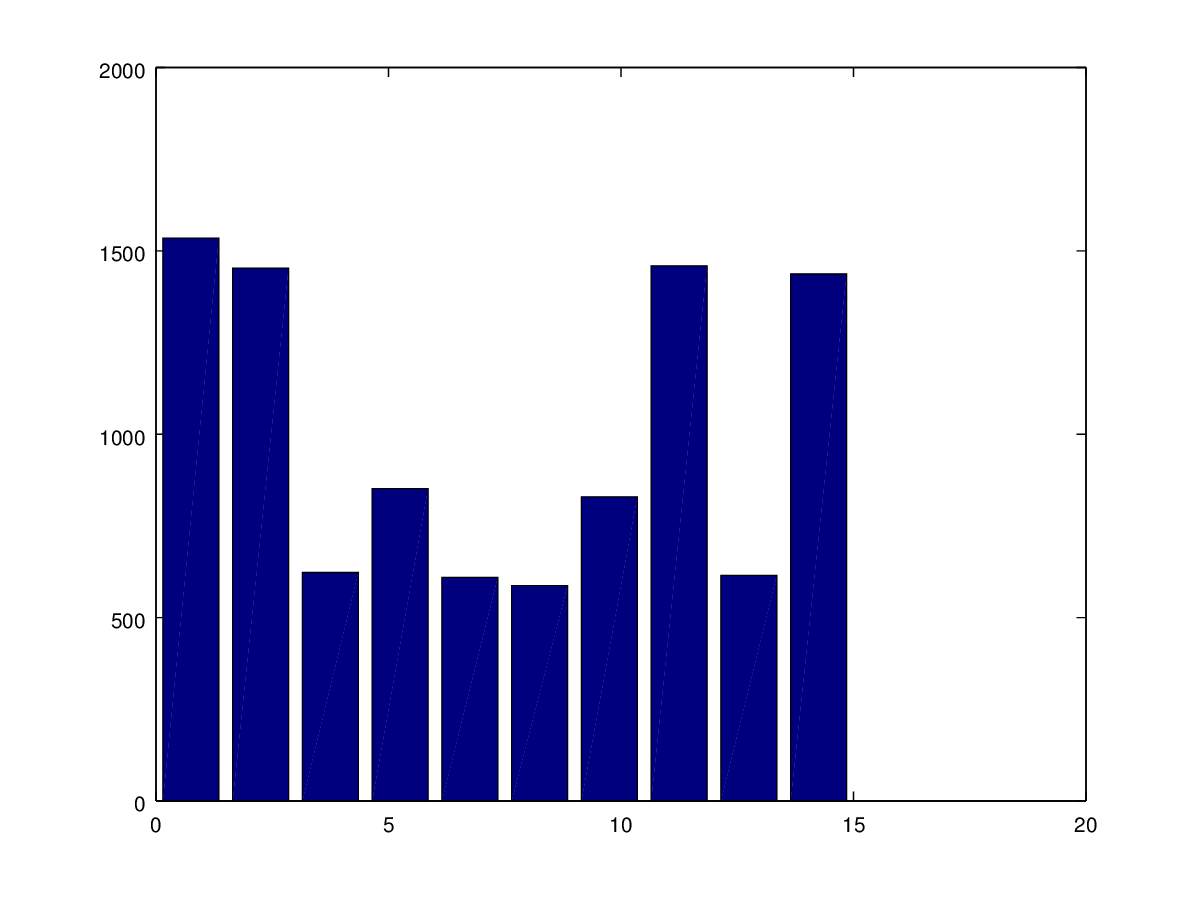
\includegraphics[scale=0.5]{boolfunctions2.png}\\
	\texttt{
f8 min 568\\
f10 max 918
	}\\
	$\frac{918}{568} = 1.616197$\\
	\\
	\textbf{Code:}
	\begin{lstlisting}
0;
function e = exec1(w1,w2,w3,t1,t2)
  if ((w1*t1 + w2*t2 + w3) >= 0)
     e = 1;
   else
     e = 0;
   endif
endfunction

function f = getBoolFunc(w1,w2,w3)
  e1 = exec1(w1,w2,w3,-1,-1);
  e2 = exec1(w1,w2,w3,-1,1);
  e3 = exec1(w1,w2,w3,1,-1);
  e4 = exec1(w1,w2,w3,1,1);
  
  f = e1*2^0 + e2*2^1 + e3*2^2 + e4*2^3;
endfunction

n = 10000;
rndweights = zeros(n,3);
ff = zeros(16,1);
functions = zeros(n,1);
[h,w] = size(rndweights);

for i = 1:h
  rndweights(i,:) = -1 + 2*rand(1,3);
endfor

for i = 1:h
  w1 = rndweights(i,1);
  w2 = rndweights(i,2);
  w3 = rndweights(i,3);
  f = getBoolFunc(w1,w2,w3);
  functions(i,1) = f;
  ff(f+1,1) += 1;
endfor

hist(functions,16);
m = max(ff);
for i = 1:16
  if ff(i,1) < m && ff(i,1) > 0
    m = ff(i,1);
  endif
endfor
ff
fprintf("min %d  max %d\n",m,max(ff));
	\end{lstlisting}
\end{document}